\hoffset-.5cm
\voffset-1cm

\documentclass{article}

\usepackage{amsmath,amssymb,amsfonts}
\usepackage{a4}
\usepackage{graphicx}

\addtolength{\leftmargin}{-3cm}
\addtolength{\textwidth}{2cm}

\title{PL: a GAP 4 package for piecewise-linear topology and mathematical physics}
\author{Alexey Korepanov, Igor Korepanov, Nurlan Sadykov}
\date{April 27, 2011}

\begin{document}

\maketitle

\tableofcontents


\section{Loading the package}

Extract the package \verb|PL| in your \verb|pkg| directory and then write
\begin{verbatim}
gap> LoadPackage("PL");
\end{verbatim}
or, alternatively, put the line \verb|LoadPackage("PL");| in your \verb|.gaprc| file or the like.


\section{PL ball complexes and how they are represented in~\tt{PL}}

\subsection{Definition of PL ball complex}

Piecewise-linear, or simply PL, ball complexes are, at least at this moment, the central objects with which our package~\verb|PL| deals.

First, a ball complex (see e.g.~\cite{Mnev}) is, simply speaking, a kind of cell complex but such where all \emph{closed} cells (${}={}$balls) are \emph{embedded}. In particular, their boundaries are genuine spheres, not crumpled/folded. The formal definition of PL ball complex reads:

\begin{quotation}
A PL ball complex is a pair $(X, U)$, where $X$ is a compact Euclidean polyhedron and $U$ is a covering of $X$ by closed PL-balls such that the following axioms are satisfied:
\begin{itemize}
\item the relative interiors of balls from~$U$ form a partition of~$X$,
\item the boundary of each ball from~$U$ is a union of balls from~$U$.
\end{itemize}
\end{quotation}

We also call PL ball complexes ``polytopes'', for brevity, hence prefix ``Pol'' in the names of some of our functions.

\subsection{Representation of a PL ball complex}

A PL-ball complex is defined up to PL-homeomorphism only by the combinatorics of adjunctions of its balls. Due to this, we represent them combinatorially in the following way.

First, we assume that all vertices in the complex are numbered from 1 to their total number~$N_0$. Hence, in this sense, the 0-skeleton of the complex is described. Next, assuming that the $k$-skeleton is already given, which implies (in particular) the numeration of all $k$-cells, we describe the $(k+1)$-skeleton as the list of all $(k+1)$-cells, each of which, in its turn, is the set of numbers of $k$-cells in its boundary. Then we compose the list of length~$n$, where $n$~is the dimension of the complex, whose elements are lists of 1-, ..., $n$-cells.

Thus, a three-dimensional ball $B^3$ can be represented by the following PL ball complex with two vertices 1 and~2:
\begin{verbatim}
[
  [ [1,2], [1,2] ], # two one-dimensional simplexes, each with
                    # ends 1 and 2, of which the first is referred to
                    # in the next line as 1, the second - as 2;
  [ [1,2], [1,2] ], # two disks - bigons - bounded each by
                    # one-dimensional simplexes 1 and 2;
  [ [1,2] ]         # the three-ball bounded by bigons 1 and 2
]
\end{verbatim}
This is depicted in Figure~\ref{fig:B3}.
\begin{figure}
\centering
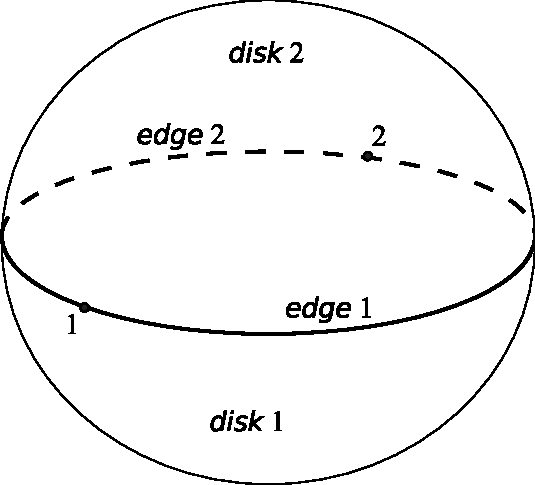
\includegraphics[scale=.5]{Ris_E_1.pdf}
\caption{Three-dimensional ball as a PL ball complex}
\label{fig:B3}
\end{figure}

Actually, we add a list of vertices with their names or something like that in the beginning of the above ball complex representation. For instance, our function \verb|ballAB(|$n$\verb|)| calls them \verb|"A"| and~\verb|"B"|. So, our GAP representation of the ball in Figure~\ref{fig:B3} is the following record:
\begin{verbatim}
gap> ballAB(3);  
rec( vertices := [ "A", "B" ], 
  faces := [ [ [ 1, 2 ], [ 1, 2 ] ], [ [ 1, 2 ], [ 1, 2 ] ], [ [ 1, 2 ] ] ] 
 )
\end{verbatim}


\section{Available functions}

\subsection{Combinatorics}

\begin{verbatim}
DeclareGlobalFunction( "PolBnd" );
# Creates an index of boundary faces of face [d,fn] of complex s
# <result>[i] --- index of (i-1)-dimensional faces of s which are 
# in the boundary of [d,fn]
# Input data: polytope, d, fn

DeclareGlobalFunction( "SostavFace" );
# almost the same as PolBnd, but written by another author 
# and having slightly different syntax:
# input data: polytope, address, where address is the list [d,fn]

DeclareGlobalFunction( "PolFaceVertices" );
# function returning set of vertices (as numbers) bounding given face of complex
# s for complex, d for dimension of the face, f for number of the face

DeclareGlobalFunction( "PolCheckComb" );
# check if a face of given complex is combinatorial complex
# that is, whether every its subface of lower dimension is uniquely
# determined by its vertices (and dimension)
# input: complex p, face dimension d and face number fn

DeclareGlobalFunction( "PolProduct" );
# Cartesian product of two polytopes

DeclareGlobalFunction( "PolProductSyms" );
# Cartesian product of two polytopes with symmetries of 
# multipliers transferred to it.
# First go the symmetries of the first multiplier, then - the second

DeclareGlobalFunction( "PolProductSymsDict" );
# Cartesian product of two polytopes with symmetries of 
# multipliers transferred to it.
# First go the symmetries of the first multiplier, then - the second.
# Also returns the face dictionary.

DeclareGlobalFunction( "PolTriangulate" );
# triangulating a polytope ( = ball complex)

DeclareGlobalFunction( "OrientTriangulated" );
# Function computes consistent orientation on simplices of greatest dimension
# on a given triangulated complex s.
# Returns array of -1,1-s which correspond to the orientation of simplices 
# of greatest dimension of s

DeclareGlobalFunction( "PolInnerFaces" );
# build index of inner faces of given polytope complex
# (!) <returned value>[i] --- set of inner faces of dimension (i-1)
# Any face is outer if it has at most 1 adjacent face of higher dimension
# or if it lies in the boundary of such a face.
# And inner faces are not outer faces.

DeclareGlobalFunction( "PolDoubleCone" );
# Make a double cone with vertices V1 and V2 over the given polytope p

DeclareGlobalFunction( "PolCylinder" );
# Maybe not needed in view of the existence of PolProduct(Syms), but anyhow:
# triangulates a polytope M and creates a triangulated cylinder over it;
# in the list for faces of any dimensions (including vertices),
# first go two identical copies of triangulated M -   M x {0}  and  M x {1}
# Also, <result>.l[i+1] is the number of i-faces in the triangulated M

DeclareGlobalFunction( "MaxTree" );
# finds a maximal tree in the 1-skeleton of a polytope as a list of edges

DeclareGlobalFunction( "CellOrient" );
# Argument: ball complex  p .
# provides inductively some orientations for cells of dimensions 1..(dim p) 
# as consistent orientations of their faces.

DeclareGlobalFunction( "PolOrient" );
# Argument: ball complex  p of dimension >1.
# If  p  is orientable, gives a consistent orientation of n-faces (n= dim p),
# otherwise returns fail

DeclareGlobalFunction( "BoundaryComponents" );
# Argument: ball complex  p of dimension >1.
# Output: list of boundary components, each being the list of its (n-1)-faces

DeclareGlobalFunction( "BoundaryComponentsAsPolytopes" );
# Argument: ball complex  p of dimension >1.
# Output: list of boundary components, each represented as a polytope

DeclareGlobalFunction( "Slovo" );
# Arguments: two lists, both corresponding to a certain 2-face.
# The first list consists of its edges represented 
# in the standard way as sets of their vertices.
# The second list consists of group elements ascribed to these edges.
# Output: a word ("slovo" in Russian) corresponding to the 2-face

DeclareGlobalFunction( "FundGroup" );
# Computes the fundamental group of the given polytope

DeclareGlobalFunction( "PolMinusFace" );
# cuts out a neighborhood of a face with given address from polytope
# Arguments: p, [d, fn]

DeclareGlobalFunction( "PolMinusPol" );
# cuts out a neighborhood of a subpolytope from polytope
# Arguments: p - polytope, sp=rec(vertices:=[...],faces:=[...])  
#  - addresses of cut out faces
# sp.faces[i] is the list of numbers of i-faces to be removed.
# output: new polytope новый политоп
# dependencies: PolMinusFace.g

DeclareGlobalFunction( "DelFace" );
# an auxiliary function: cuts out a face with address [k, m] 
# from polytope  p, shifting back all necessary numbers. 
# This returns a polytope-like structure which
# may not be ball complex, but it works well if employed skillfully.
# Arguments: p, address

DeclareGlobalFunction( "PolSimplify1" );
# symplifies a polytope by merging two k-faces when possible, starting from k=n
# and down to k=1. If actual simplification is achieved, try this again and so on.
# Probably, there will be "PolSymplify2" and so on in the future.

DeclareGlobalFunction( "PolFactorInvolution" );
# PolFactorInvolution := function( p, invol )
# p is the polytope with symmetries
# invol is such a list of some of its symmetries (repetitions possible)
# that it is known that the product of symmetries in s is an involution
# returns the factored polytope
\end{verbatim}


\subsection{Polytopes}

\begin{verbatim}
# Define a polytope somehow

DeclareGlobalVariable( "Simplex1", "line segment - simplex of dimension 1" );

DeclareGlobalVariable( "Simplex2", "triangle - simplex of dimension 2" );

DeclareGlobalVariable( "Simplex3", "tetrahedron - simplex of dimension 2" );

DeclareGlobalVariable( "3sq", "triple square" );

DeclareGlobalVariable( "T2", "2-dimensional torus, 4 symmetries: 2 translations, 
x -> -x in both coordinates together, rotation" );

DeclareGlobalVariable( "Cube", "cube" );

DeclareGlobalVariable( "S3cubic", "sphere S^3 as two cubes" );

DeclareGlobalVariable( "Sphere1", "circle, with two vertices and symmetries" );

DeclareGlobalVariable( "Sphere2", "sphere S^2 made of two triangles" );

DeclareGlobalVariable( "Sphere4", "sphere S^4 made of two 4-simplices" );

DeclareGlobalVariable( "Disk3", "disk D^3 with two triangles as boundary 
and one vertex, namely A, inside" );

DeclareGlobalVariable( "3cubes", "non-manifold: 3 cubes all 
glued at the same boundary" );

DeclareGlobalVariable( "Bigon", "bigon" );

DeclareGlobalVariable( "3pillow", "3-d pillow" );

DeclareGlobalVariable( "3pillow1", "3-d pillow - with another order on vertices" );

DeclareGlobalVariable( "Lantern", "lantern - D^3 with 3 faces" );

DeclareGlobalVariable( "DoubleLantern", "double lantern 
(interior and exterior) with 4 edges" );

DeclareGlobalVariable( "MobiusBand", "Mobius band made of two squares" );

############################################################# now functions

DeclareGlobalFunction( "Lens" ); # 3-d lens spaces; usage: Lens(7,1)

DeclareGlobalFunction( "PolPrint" ); # print all the faces of 
simplitial complex in terms of names of vertices

DeclareGlobalFunction( "ballAB" ); # a ball of dimension n 
# and just two vertices A and B

DeclareGlobalFunction( "sphereAB" ); # a sphere of dimension n 
# and just two vertices A and B

DeclareGlobalFunction( "KummerSurface" ); 
# KummerSurface() makes the Kummer surface
\end{verbatim}

\subsection{Grassmann}

\begin{verbatim}
DeclareGlobalFunction( "GrassmannSum" );
# GrassmannSum := function( x,y )
# x and y are records representing elements of a Grassmann algebra
# RecNames are "monomials" and "coeffs"
# "monomials" is a list of monomials, each element being 
# a product of Grassmann generators
# if this element is [3,4], then it is (generator no. 3)*(generator no. 4)
# and these elements *must* be sets!
# "coeffs" is the list of coefficients at corresponding products

DeclareGlobalFunction( "GrassmannMonomialsProduct" );
# GrassmannMonomialsProduct := function( x1,x2 )
# x1 = [<monomial>,<coefficient>], x2 similarly
# returns their product written in a similar way

DeclareGlobalFunction( "GrassmannProduct" );
# GrassmannProduct := function( x,y )
# x and y are records representing elements of Grassmann algebra
# returns x*y

DeclareGlobalFunction( "BerezinIntegral" );
# BerezinIntegral := function( x, a )
# x is a record representing Grassmann algebra element
# a is a (number of) Grassmann variable
# returns the record representing the integral

DeclareGlobalFunction( "BerezinMultipleIntegral" );
# BerezinMultipleIntegral := function( x, l )
# x is a record representing Grassmann algebra element
# l is a list of (numbers of) Grassmann variables
# integration goes first in the first variable, then the second etc.
# returns the record representing the integral
\end{verbatim}

\subsection{Building chain complexes (compbuild)}

\begin{verbatim}
DeclareGlobalFunction( "Matrices4dAffineTriangulated" );
# Returns a structure with matrices f2,f3_full,f4_full,f5 
# and supplementary information
# for given polytope complex of dimension 4. Arguments:
# p is the initial polytope (not necessarily triangulated),
# num is a logical (I mean Boolean) variable: if num is true, 
# the coordinates z[i] are numbers,
# f is the function determining the coordinates: z[i]=f(i). 
# So, if num is false f does not affect the result.
# (!) Does not work if some matrices are empty

DeclareGlobalFunction( "f3E4" );
# Arguments: 4-simplex  four_simplex = [i1,i2,i3,i4,i5], 
# its 2-face  two_face  and edge  edge .
# Computes the (partial) derivative of the squared sine of dihedral angle 
# at two_face wrt squared edge length

DeclareGlobalFunction( "Matrices4dEuclid4" );
# return structure with matrices f2_full,f3_FULL,f4_full,f5
# constructed using Euclidean 4-dimensional geometry
# and supplementary information
# for given 4-manifold with one-component boundary. Arguments:
# p is the initial polytope (not necessarily triangulated),
# coord is the list [w,x,y,z], where w,x,y,z are 
# long enough lists of rational numbers
# and such that no five vertices lie in a 3-plane
\end{verbatim}

\subsection{Calculations with chain complexes (compcalc)}


\subsection{Knots}

\begin{verbatim}
DeclareGlobalVariable( "Trefoil", "diagram of the trefoil knot" );

DeclareGlobalVariable( "Figure8", "diagram of the figure-eight knot" );

DeclareGlobalVariable( "Unknot", " a diagram for the unknot" );

DeclareGlobalVariable( "Knot7_7", "diagram of the knot 7_7" );

#################################################################
#########################   and now functions
#################################################################


DeclareGlobalFunction( "LeftRight" );
# auxiliary function for knots calculations

DeclareGlobalFunction( "SectionLR" );
# auxiliary function for knots calculations

DeclareGlobalFunction( "Diagonal2" );
# auxiliary function for knots calculations
# or maybe more interesting...

DeclareGlobalFunction( "KnotInD3" );
# placing knot in D^3

DeclareGlobalFunction( "KnotGroupD3" );
# computes knot group from knot
\end{verbatim}




\section{Example of a test calculation}\label{sec:test}

We will check that if we take a 6-dimensional sphere~$A=S^6$ and remove from it a tubular neighborhood of a non-knotted 4-dimensional sphere~$B=S^4$, then the fundamental group af the resulting manifold is~$\mathbb Z$.

First, look at our realization of~$S^6$:
\begin{verbatim}
gap> A := sphereAB(6);
rec( vertices := [ "A", "B" ], 
  faces := [ [ [ 1, 2 ], [ 1, 2 ] ], [ [ 1, 2 ], [ 1, 2 ] ], 
      [ [ 1, 2 ], [ 1, 2 ] ], [ [ 1, 2 ], [ 1, 2 ] ], [ [ 1, 2 ], [ 1, 2 ] ], 
      [ [ 1, 2 ], [ 1, 2 ] ] ] )
\end{verbatim}
Then we prepare $B$ in the following way:
\begin{verbatim}
gap> B := rec( vertices := [1,2], faces := [ [1,2],[1,2],[1,2],[1,2] ] );
rec( vertices := [ 1, 2 ], 
  faces := [ [ 1, 2 ], [ 1, 2 ], [ 1, 2 ], [ 1, 2 ] ] )
\end{verbatim}
Note the difference with~$A$: here we provide \emph{numbers} of vertices and faces from those \emph{already listed} in~$A$. 

Now ``polytope minus polytope'', or, to be exact, polytope~$A$ minus tubular neighborhood of~$B$. The end of the result is on page~\pageref{endS6minusS4}, just go there and find some interesting continuation:
\begin{verbatim}
gap> C := PolMinusPol( A, B );
rec( vertices := [ "A", "B", 3, 4, 5, 6, 7, 8, 9, 10, 11, 12, 13, 14, 15, 
      16, 17, 18, 19, 20, 21, 22, 23, 24, 25, 26, 27, 28, 29, 30, 31, 32, 
      33, 34, 35, 36, 37, 38, 39, 40, 41, 42, 43, 44, 45, 46, 47, 48, 49, 
      50, 51, 52, 53, 54, 55, 56, 57, 58, 59, 60, 61, 62, 63, 64 ], 
  faces := 
    [ [ [ 3, 34 ], [ 4, 35 ], [ 5, 36 ], [ 6, 37 ], [ 7, 38 ], [ 8, 39 ], 
          [ 9, 40 ], [ 10, 41 ], [ 11, 42 ], [ 12, 43 ], [ 13, 44 ], 
          [ 14, 45 ], [ 15, 46 ], [ 16, 47 ], [ 17, 48 ], [ 18, 49 ], 
          [ 19, 50 ], [ 20, 51 ], [ 21, 52 ], [ 22, 53 ], [ 23, 54 ], 
          [ 24, 55 ], [ 25, 56 ], [ 26, 57 ], [ 27, 58 ], [ 28, 59 ], 
          [ 29, 60 ], [ 30, 61 ], [ 31, 62 ], [ 32, 63 ], [ 33, 64 ], 
          [ 1, 2 ], [ 5, 20 ], [ 6, 21 ], [ 7, 22 ], [ 8, 23 ], [ 9, 24 ], 
          [ 10, 25 ], [ 11, 26 ], [ 12, 27 ], [ 13, 28 ], [ 14, 29 ], 
          [ 15, 30 ], [ 16, 31 ], [ 17, 32 ], [ 18, 33 ], [ 2, 19 ], 
          [ 3, 4 ], [ 7, 14 ], [ 8, 15 ], [ 9, 16 ], [ 10, 17 ], 
          [ 11, 18 ], [ 12, 19 ], [ 4, 13 ], [ 5, 6 ], [ 9, 12 ], 
          [ 10, 13 ], [ 6, 11 ], [ 7, 8 ], [ 8, 11 ], [ 9, 10 ], 
          [ 10, 11 ], [ 10, 11 ], [ 8, 9 ], [ 8, 9 ], [ 6, 7 ], [ 12, 13 ], 
          [ 6, 13 ], [ 6, 13 ], [ 7, 12 ], [ 7, 12 ], [ 16, 19 ], 
          [ 4, 17 ], [ 5, 18 ], [ 14, 15 ], [ 15, 18 ], [ 16, 17 ], 
          [ 17, 18 ], [ 17, 18 ], [ 15, 16 ], [ 15, 16 ], [ 5, 14 ], 
          [ 4, 19 ], [ 4, 5 ], [ 4, 5 ], [ 14, 19 ], [ 14, 19 ], 
          [ 22, 29 ], [ 23, 30 ], [ 24, 31 ], [ 25, 32 ], [ 26, 33 ], 
          [ 2, 27 ], [ 3, 28 ], [ 20, 21 ], [ 24, 27 ], [ 25, 28 ], 
          [ 21, 26 ], [ 22, 23 ], [ 23, 26 ], [ 24, 25 ], [ 25, 26 ], 
          [ 25, 26 ], [ 23, 24 ], [ 23, 24 ], [ 21, 22 ], [ 27, 28 ], 
          [ 21, 28 ], [ 21, 28 ], [ 22, 27 ], [ 22, 27 ], [ 2, 31 ], 
          [ 3, 32 ], [ 20, 33 ], [ 29, 30 ], [ 30, 33 ], [ 31, 32 ], 
          [ 32, 33 ], [ 32, 33 ], [ 30, 31 ], [ 30, 31 ], [ 20, 29 ], 
          [ 2, 3 ], [ 3, 20 ], [ 3, 20 ], [ 2, 29 ], [ 2, 29 ], [ 36, 51 ], 
          [ 37, 52 ], [ 38, 53 ], [ 39, 54 ], [ 40, 55 ], [ 41, 56 ], 
          [ 42, 57 ], [ 43, 58 ], [ 44, 59 ], [ 45, 60 ], [ 46, 61 ], 
          [ 47, 62 ], [ 48, 63 ], [ 49, 64 ], [ 1, 50 ], [ 34, 35 ], 
          [ 38, 45 ], [ 39, 46 ], [ 40, 47 ], [ 41, 48 ], [ 42, 49 ], 
          [ 43, 50 ], [ 35, 44 ], [ 36, 37 ], [ 40, 43 ], [ 41, 44 ], 
          [ 37, 42 ], [ 38, 39 ], [ 39, 42 ], [ 40, 41 ], [ 41, 42 ], 
          [ 41, 42 ], [ 39, 40 ], [ 39, 40 ], [ 37, 38 ], [ 43, 44 ], 
          [ 37, 44 ], [ 37, 44 ], [ 38, 43 ], [ 38, 43 ], [ 47, 50 ], 
          [ 35, 48 ], [ 36, 49 ], [ 45, 46 ], [ 46, 49 ], [ 47, 48 ], 
          [ 48, 49 ], [ 48, 49 ], [ 46, 47 ], [ 46, 47 ], [ 36, 45 ], 
          [ 35, 50 ], [ 35, 36 ], [ 35, 36 ], [ 45, 50 ], [ 45, 50 ], 
          [ 53, 60 ], [ 54, 61 ], [ 55, 62 ], [ 56, 63 ], [ 57, 64 ], 
          [ 1, 58 ], [ 34, 59 ], [ 51, 52 ], [ 55, 58 ], [ 56, 59 ], 
          [ 52, 57 ], [ 53, 54 ], [ 54, 57 ], [ 55, 56 ], [ 56, 57 ], 
          [ 56, 57 ], [ 54, 55 ], [ 54, 55 ], [ 52, 53 ], [ 58, 59 ], 
          [ 52, 59 ], [ 52, 59 ], [ 53, 58 ], [ 53, 58 ], [ 1, 62 ], 
          [ 34, 63 ], [ 51, 64 ], [ 60, 61 ], [ 61, 64 ], [ 62, 63 ], 
          [ 63, 64 ], [ 63, 64 ], [ 61, 62 ], [ 61, 62 ], [ 51, 60 ], 
          [ 1, 34 ], [ 34, 51 ], [ 34, 51 ], [ 1, 60 ], [ 1, 60 ] ], 
      [ [ 3, 18, 33, 129 ], [ 4, 19, 34, 130 ], [ 5, 20, 35, 131 ], 
          [ 6, 21, 36, 132 ], [ 7, 22, 37, 133 ], [ 8, 23, 38, 134 ], 
          [ 9, 24, 39, 135 ], [ 10, 25, 40, 136 ], [ 11, 26, 41, 137 ], 
          [ 12, 27, 42, 138 ], [ 13, 28, 43, 139 ], [ 14, 29, 44, 140 ], 
          [ 15, 30, 45, 141 ], [ 16, 31, 46, 142 ], [ 17, 32, 47, 143 ], 
          [ 1, 2, 48, 144 ], [ 5, 12, 49, 145 ], [ 6, 13, 50, 146 ], 
          [ 7, 14, 51, 147 ], [ 8, 15, 52, 148 ], [ 9, 16, 53, 149 ], 
          [ 10, 17, 54, 150 ], [ 2, 11, 55, 151 ], [ 3, 4, 56, 152 ], 
          [ 7, 10, 57, 153 ], [ 8, 11, 58, 154 ], [ 4, 9, 59, 155 ], 
          [ 5, 6, 60, 156 ], [ 6, 9, 61, 157 ], [ 7, 8, 62, 158 ], 
          [ 8, 9, 63, 159 ], [ 8, 9, 64, 160 ], [ 6, 7, 65, 161 ], 
          [ 6, 7, 66, 162 ], [ 4, 5, 67, 163 ], [ 10, 11, 68, 164 ], 
          [ 4, 11, 69, 165 ], [ 4, 11, 70, 166 ], [ 5, 10, 71, 167 ], 
          [ 5, 10, 72, 168 ], [ 14, 17, 73, 169 ], [ 2, 15, 74, 170 ], 
          [ 3, 16, 75, 171 ], [ 12, 13, 76, 172 ], [ 13, 16, 77, 173 ], 
          [ 14, 15, 78, 174 ], [ 15, 16, 79, 175 ], [ 15, 16, 80, 176 ], 
          [ 13, 14, 81, 177 ], [ 13, 14, 82, 178 ], [ 3, 12, 83, 179 ], 
          [ 2, 17, 84, 180 ], [ 2, 3, 85, 181 ], [ 2, 3, 86, 182 ], 
          [ 12, 17, 87, 183 ], [ 12, 17, 88, 184 ], [ 20, 27, 89, 185 ], 
          [ 21, 28, 90, 186 ], [ 22, 29, 91, 187 ], [ 23, 30, 92, 188 ], 
          [ 24, 31, 93, 189 ], [ 25, 32, 94, 190 ], [ 1, 26, 95, 191 ], 
          [ 18, 19, 96, 192 ], [ 22, 25, 97, 193 ], [ 23, 26, 98, 194 ], 
          [ 19, 24, 99, 195 ], [ 20, 21, 100, 196 ], [ 21, 24, 101, 197 ], 
          [ 22, 23, 102, 198 ], [ 23, 24, 103, 199 ], [ 23, 24, 104, 200 ], 
          [ 21, 22, 105, 201 ], [ 21, 22, 106, 202 ], [ 19, 20, 107, 203 ], 
          [ 25, 26, 108, 204 ], [ 19, 26, 109, 205 ], [ 19, 26, 110, 206 ], 
          [ 20, 25, 111, 207 ], [ 20, 25, 112, 208 ], [ 29, 32, 113, 209 ], 
          [ 1, 30, 114, 210 ], [ 18, 31, 115, 211 ], [ 27, 28, 116, 212 ], 
          [ 28, 31, 117, 213 ], [ 29, 30, 118, 214 ], [ 30, 31, 119, 215 ], 
          [ 30, 31, 120, 216 ], [ 28, 29, 121, 217 ], [ 28, 29, 122, 218 ], 
          [ 18, 27, 123, 219 ], [ 1, 32, 124, 220 ], [ 1, 18, 125, 221 ], 
          [ 1, 18, 126, 222 ], [ 27, 32, 127, 223 ], [ 27, 32, 128, 224 ], 
          [ 35, 42, 49, 89 ], [ 36, 43, 50, 90 ], [ 37, 44, 51, 91 ], 
          [ 38, 45, 52, 92 ], [ 39, 46, 53, 93 ], [ 40, 47, 54, 94 ], 
          [ 41, 48, 55, 95 ], [ 33, 34, 56, 96 ], [ 37, 40, 57, 97 ], 
          [ 38, 41, 58, 98 ], [ 34, 39, 59, 99 ], [ 35, 36, 60, 100 ], 
          [ 36, 39, 61, 101 ], [ 37, 38, 62, 102 ], [ 38, 39, 63, 103 ], 
          [ 38, 39, 64, 104 ], [ 36, 37, 65, 105 ], [ 36, 37, 66, 106 ], 
          [ 34, 35, 67, 107 ], [ 40, 41, 68, 108 ], [ 34, 41, 69, 109 ], 
          [ 34, 41, 70, 110 ], [ 35, 40, 71, 111 ], [ 35, 40, 72, 112 ], 
          [ 44, 47, 73, 113 ], [ 45, 48, 74, 114 ], [ 33, 46, 75, 115 ], 
          [ 42, 43, 76, 116 ], [ 43, 46, 77, 117 ], [ 44, 45, 78, 118 ], 
          [ 45, 46, 79, 119 ], [ 45, 46, 80, 120 ], [ 43, 44, 81, 121 ], 
          [ 43, 44, 82, 122 ], [ 33, 42, 83, 123 ], [ 47, 48, 84, 124 ], 
          [ 33, 48, 85, 125 ], [ 33, 48, 86, 126 ], [ 42, 47, 87, 127 ], 
          [ 42, 47, 88, 128 ], [ 51, 54, 57, 73 ], [ 52, 55, 58, 74 ], 
          [ 53, 56, 59, 75 ], [ 49, 50, 60, 76 ], [ 50, 53, 61, 77 ], 
          [ 51, 52, 62, 78 ], [ 52, 53, 63, 79 ], [ 52, 53, 64, 80 ], 
          [ 50, 51, 65, 81 ], [ 50, 51, 66, 82 ], [ 49, 56, 67, 83 ], 
          [ 54, 55, 68, 84 ], [ 55, 56, 69, 85 ], [ 55, 56, 70, 86 ], 
          [ 49, 54, 71, 87 ], [ 49, 54, 72, 88 ], [ 59, 60, 61, 67 ], 
          [ 57, 58, 62, 68 ], [ 58, 59, 63, 69 ], [ 58, 59, 64, 70 ], 
          [ 57, 60, 65, 71 ], [ 57, 60, 66, 72 ], [ 61, 62, 63, 65 ], 
          [ 61, 62, 64, 66 ], [ 67, 68, 69, 71 ], [ 67, 68, 70, 72 ], 
          [ 75, 76, 77, 83 ], [ 73, 74, 78, 84 ], [ 74, 75, 79, 85 ], 
          [ 74, 75, 80, 86 ], [ 73, 76, 81, 87 ], [ 73, 76, 82, 88 ], 
          [ 77, 78, 79, 81 ], [ 77, 78, 80, 82 ], [ 83, 84, 85, 87 ], 
          [ 83, 84, 86, 88 ], [ 91, 94, 97, 113 ], [ 92, 95, 98, 114 ], 
          [ 93, 96, 99, 115 ], [ 89, 90, 100, 116 ], [ 90, 93, 101, 117 ], 
          [ 91, 92, 102, 118 ], [ 92, 93, 103, 119 ], [ 92, 93, 104, 120 ], 
          [ 90, 91, 105, 121 ], [ 90, 91, 106, 122 ], [ 89, 96, 107, 123 ], 
          [ 94, 95, 108, 124 ], [ 95, 96, 109, 125 ], [ 95, 96, 110, 126 ], 
          [ 89, 94, 111, 127 ], [ 89, 94, 112, 128 ], [ 99, 100, 101, 107 ],
          [ 97, 98, 102, 108 ], [ 98, 99, 103, 109 ], [ 98, 99, 104, 110 ], 
          [ 97, 100, 105, 111 ], [ 97, 100, 106, 112 ], 
          [ 101, 102, 103, 105 ], [ 101, 102, 104, 106 ], 
          [ 107, 108, 109, 111 ], [ 107, 108, 110, 112 ], 
          [ 115, 116, 117, 123 ], [ 113, 114, 118, 124 ], 
          [ 114, 115, 119, 125 ], [ 114, 115, 120, 126 ], 
          [ 113, 116, 121, 127 ], [ 113, 116, 122, 128 ], 
          [ 117, 118, 119, 121 ], [ 117, 118, 120, 122 ], 
          [ 123, 124, 125, 127 ], [ 123, 124, 126, 128 ], 
          [ 131, 138, 145, 185 ], [ 132, 139, 146, 186 ], 
          [ 133, 140, 147, 187 ], [ 134, 141, 148, 188 ], 
          [ 135, 142, 149, 189 ], [ 136, 143, 150, 190 ], 
          [ 137, 144, 151, 191 ], [ 129, 130, 152, 192 ], 
          [ 133, 136, 153, 193 ], [ 134, 137, 154, 194 ], 
          [ 130, 135, 155, 195 ], [ 131, 132, 156, 196 ], 
          [ 132, 135, 157, 197 ], [ 133, 134, 158, 198 ], 
          [ 134, 135, 159, 199 ], [ 134, 135, 160, 200 ], 
          [ 132, 133, 161, 201 ], [ 132, 133, 162, 202 ], 
          [ 130, 131, 163, 203 ], [ 136, 137, 164, 204 ], 
          [ 130, 137, 165, 205 ], [ 130, 137, 166, 206 ], 
          [ 131, 136, 167, 207 ], [ 131, 136, 168, 208 ], 
          [ 140, 143, 169, 209 ], [ 141, 144, 170, 210 ], 
          [ 129, 142, 171, 211 ], [ 138, 139, 172, 212 ], 
          [ 139, 142, 173, 213 ], [ 140, 141, 174, 214 ], 
          [ 141, 142, 175, 215 ], [ 141, 142, 176, 216 ], 
          [ 139, 140, 177, 217 ], [ 139, 140, 178, 218 ], 
          [ 129, 138, 179, 219 ], [ 143, 144, 180, 220 ], 
          [ 129, 144, 181, 221 ], [ 129, 144, 182, 222 ], 
          [ 138, 143, 183, 223 ], [ 138, 143, 184, 224 ], 
          [ 147, 150, 153, 169 ], [ 148, 151, 154, 170 ], 
          [ 149, 152, 155, 171 ], [ 145, 146, 156, 172 ], 
          [ 146, 149, 157, 173 ], [ 147, 148, 158, 174 ], 
          [ 148, 149, 159, 175 ], [ 148, 149, 160, 176 ], 
          [ 146, 147, 161, 177 ], [ 146, 147, 162, 178 ], 
          [ 145, 152, 163, 179 ], [ 150, 151, 164, 180 ], 
          [ 151, 152, 165, 181 ], [ 151, 152, 166, 182 ], 
          [ 145, 150, 167, 183 ], [ 145, 150, 168, 184 ], 
          [ 155, 156, 157, 163 ], [ 153, 154, 158, 164 ], 
          [ 154, 155, 159, 165 ], [ 154, 155, 160, 166 ], 
          [ 153, 156, 161, 167 ], [ 153, 156, 162, 168 ], 
          [ 157, 158, 159, 161 ], [ 157, 158, 160, 162 ], 
          [ 163, 164, 165, 167 ], [ 163, 164, 166, 168 ], 
          [ 171, 172, 173, 179 ], [ 169, 170, 174, 180 ], 
          [ 170, 171, 175, 181 ], [ 170, 171, 176, 182 ], 
          [ 169, 172, 177, 183 ], [ 169, 172, 178, 184 ], 
          [ 173, 174, 175, 177 ], [ 173, 174, 176, 178 ], 
          [ 179, 180, 181, 183 ], [ 179, 180, 182, 184 ], 
          [ 187, 190, 193, 209 ], [ 188, 191, 194, 210 ], 
          [ 189, 192, 195, 211 ], [ 185, 186, 196, 212 ], 
          [ 186, 189, 197, 213 ], [ 187, 188, 198, 214 ], 
          [ 188, 189, 199, 215 ], [ 188, 189, 200, 216 ], 
          [ 186, 187, 201, 217 ], [ 186, 187, 202, 218 ], 
          [ 185, 192, 203, 219 ], [ 190, 191, 204, 220 ], 
          [ 191, 192, 205, 221 ], [ 191, 192, 206, 222 ], 
          [ 185, 190, 207, 223 ], [ 185, 190, 208, 224 ], 
          [ 195, 196, 197, 203 ], [ 193, 194, 198, 204 ], 
          [ 194, 195, 199, 205 ], [ 194, 195, 200, 206 ], 
          [ 193, 196, 201, 207 ], [ 193, 196, 202, 208 ], 
          [ 197, 198, 199, 201 ], [ 197, 198, 200, 202 ], 
          [ 203, 204, 205, 207 ], [ 203, 204, 206, 208 ], 
          [ 211, 212, 213, 219 ], [ 209, 210, 214, 220 ], 
          [ 210, 211, 215, 221 ], [ 210, 211, 216, 222 ], 
          [ 209, 212, 217, 223 ], [ 209, 212, 218, 224 ], 
          [ 213, 214, 215, 217 ], [ 213, 214, 216, 218 ], 
          [ 219, 220, 221, 223 ], [ 219, 220, 222, 224 ] ], 
      [ [ 3, 10, 17, 57, 97, 209 ], [ 4, 11, 18, 58, 98, 210 ], 
          [ 5, 12, 19, 59, 99, 211 ], [ 6, 13, 20, 60, 100, 212 ], 
          [ 7, 14, 21, 61, 101, 213 ], [ 8, 15, 22, 62, 102, 214 ], 
          [ 9, 16, 23, 63, 103, 215 ], [ 1, 2, 24, 64, 104, 216 ], 
          [ 5, 8, 25, 65, 105, 217 ], [ 6, 9, 26, 66, 106, 218 ], 
          [ 2, 7, 27, 67, 107, 219 ], [ 3, 4, 28, 68, 108, 220 ], 
          [ 4, 7, 29, 69, 109, 221 ], [ 5, 6, 30, 70, 110, 222 ], 
          [ 6, 7, 31, 71, 111, 223 ], [ 6, 7, 32, 72, 112, 224 ], 
          [ 4, 5, 33, 73, 113, 225 ], [ 4, 5, 34, 74, 114, 226 ], 
          [ 2, 3, 35, 75, 115, 227 ], [ 8, 9, 36, 76, 116, 228 ], 
          [ 2, 9, 37, 77, 117, 229 ], [ 2, 9, 38, 78, 118, 230 ], 
          [ 3, 8, 39, 79, 119, 231 ], [ 3, 8, 40, 80, 120, 232 ], 
          [ 12, 15, 41, 81, 121, 233 ], [ 13, 16, 42, 82, 122, 234 ], 
          [ 1, 14, 43, 83, 123, 235 ], [ 10, 11, 44, 84, 124, 236 ], 
          [ 11, 14, 45, 85, 125, 237 ], [ 12, 13, 46, 86, 126, 238 ], 
          [ 13, 14, 47, 87, 127, 239 ], [ 13, 14, 48, 88, 128, 240 ], 
          [ 11, 12, 49, 89, 129, 241 ], [ 11, 12, 50, 90, 130, 242 ], 
          [ 1, 10, 51, 91, 131, 243 ], [ 15, 16, 52, 92, 132, 244 ], 
          [ 1, 16, 53, 93, 133, 245 ], [ 1, 16, 54, 94, 134, 246 ], 
          [ 10, 15, 55, 95, 135, 247 ], [ 10, 15, 56, 96, 136, 248 ], 
          [ 19, 22, 25, 41, 137, 249 ], [ 20, 23, 26, 42, 138, 250 ], 
          [ 21, 24, 27, 43, 139, 251 ], [ 17, 18, 28, 44, 140, 252 ], 
          [ 18, 21, 29, 45, 141, 253 ], [ 19, 20, 30, 46, 142, 254 ], 
          [ 20, 21, 31, 47, 143, 255 ], [ 20, 21, 32, 48, 144, 256 ], 
          [ 18, 19, 33, 49, 145, 257 ], [ 18, 19, 34, 50, 146, 258 ], 
          [ 17, 24, 35, 51, 147, 259 ], [ 22, 23, 36, 52, 148, 260 ], 
          [ 23, 24, 37, 53, 149, 261 ], [ 23, 24, 38, 54, 150, 262 ], 
          [ 17, 22, 39, 55, 151, 263 ], [ 17, 22, 40, 56, 152, 264 ], 
          [ 27, 28, 29, 35, 153, 265 ], [ 25, 26, 30, 36, 154, 266 ], 
          [ 26, 27, 31, 37, 155, 267 ], [ 26, 27, 32, 38, 156, 268 ], 
          [ 25, 28, 33, 39, 157, 269 ], [ 25, 28, 34, 40, 158, 270 ], 
          [ 29, 30, 31, 33, 159, 271 ], [ 29, 30, 32, 34, 160, 272 ], 
          [ 35, 36, 37, 39, 161, 273 ], [ 35, 36, 38, 40, 162, 274 ], 
          [ 43, 44, 45, 51, 163, 275 ], [ 41, 42, 46, 52, 164, 276 ], 
          [ 42, 43, 47, 53, 165, 277 ], [ 42, 43, 48, 54, 166, 278 ], 
          [ 41, 44, 49, 55, 167, 279 ], [ 41, 44, 50, 56, 168, 280 ], 
          [ 45, 46, 47, 49, 169, 281 ], [ 45, 46, 48, 50, 170, 282 ], 
          [ 51, 52, 53, 55, 171, 283 ], [ 51, 52, 54, 56, 172, 284 ], 
          [ 59, 62, 65, 81, 173, 285 ], [ 60, 63, 66, 82, 174, 286 ], 
          [ 61, 64, 67, 83, 175, 287 ], [ 57, 58, 68, 84, 176, 288 ], 
          [ 58, 61, 69, 85, 177, 289 ], [ 59, 60, 70, 86, 178, 290 ], 
          [ 60, 61, 71, 87, 179, 291 ], [ 60, 61, 72, 88, 180, 292 ], 
          [ 58, 59, 73, 89, 181, 293 ], [ 58, 59, 74, 90, 182, 294 ], 
          [ 57, 64, 75, 91, 183, 295 ], [ 62, 63, 76, 92, 184, 296 ], 
          [ 63, 64, 77, 93, 185, 297 ], [ 63, 64, 78, 94, 186, 298 ], 
          [ 57, 62, 79, 95, 187, 299 ], [ 57, 62, 80, 96, 188, 300 ], 
          [ 67, 68, 69, 75, 189, 301 ], [ 65, 66, 70, 76, 190, 302 ], 
          [ 66, 67, 71, 77, 191, 303 ], [ 66, 67, 72, 78, 192, 304 ], 
          [ 65, 68, 73, 79, 193, 305 ], [ 65, 68, 74, 80, 194, 306 ], 
          [ 69, 70, 71, 73, 195, 307 ], [ 69, 70, 72, 74, 196, 308 ], 
          [ 75, 76, 77, 79, 197, 309 ], [ 75, 76, 78, 80, 198, 310 ], 
          [ 83, 84, 85, 91, 199, 311 ], [ 81, 82, 86, 92, 200, 312 ], 
          [ 82, 83, 87, 93, 201, 313 ], [ 82, 83, 88, 94, 202, 314 ], 
          [ 81, 84, 89, 95, 203, 315 ], [ 81, 84, 90, 96, 204, 316 ], 
          [ 85, 86, 87, 89, 205, 317 ], [ 85, 86, 88, 90, 206, 318 ], 
          [ 91, 92, 93, 95, 207, 319 ], [ 91, 92, 94, 96, 208, 320 ], 
          [ 99, 102, 105, 121, 137, 173 ], [ 100, 103, 106, 122, 138, 174 ],
          [ 101, 104, 107, 123, 139, 175 ], [ 97, 98, 108, 124, 140, 176 ], 
          [ 98, 101, 109, 125, 141, 177 ], [ 99, 100, 110, 126, 142, 178 ], 
          [ 100, 101, 111, 127, 143, 179 ], [ 100, 101, 112, 128, 144, 180 ]
            , [ 98, 99, 113, 129, 145, 181 ], 
          [ 98, 99, 114, 130, 146, 182 ], [ 97, 104, 115, 131, 147, 183 ], 
          [ 102, 103, 116, 132, 148, 184 ], [ 103, 104, 117, 133, 149, 185 ]
            , [ 103, 104, 118, 134, 150, 186 ], 
          [ 97, 102, 119, 135, 151, 187 ], [ 97, 102, 120, 136, 152, 188 ], 
          [ 107, 108, 109, 115, 153, 189 ], [ 105, 106, 110, 116, 154, 190 ]
            , [ 106, 107, 111, 117, 155, 191 ], 
          [ 106, 107, 112, 118, 156, 192 ], [ 105, 108, 113, 119, 157, 193 ]
            , [ 105, 108, 114, 120, 158, 194 ], 
          [ 109, 110, 111, 113, 159, 195 ], [ 109, 110, 112, 114, 160, 196 ]
            , [ 115, 116, 117, 119, 161, 197 ], 
          [ 115, 116, 118, 120, 162, 198 ], [ 123, 124, 125, 131, 163, 199 ]
            , [ 121, 122, 126, 132, 164, 200 ], 
          [ 122, 123, 127, 133, 165, 201 ], [ 122, 123, 128, 134, 166, 202 ]
            , [ 121, 124, 129, 135, 167, 203 ], 
          [ 121, 124, 130, 136, 168, 204 ], [ 125, 126, 127, 129, 169, 205 ]
            , [ 125, 126, 128, 130, 170, 206 ], 
          [ 131, 132, 133, 135, 171, 207 ], [ 131, 132, 134, 136, 172, 208 ]
            , [ 139, 140, 141, 147, 153, 163 ], 
          [ 137, 138, 142, 148, 154, 164 ], [ 138, 139, 143, 149, 155, 165 ]
            , [ 138, 139, 144, 150, 156, 166 ], 
          [ 137, 140, 145, 151, 157, 167 ], [ 137, 140, 146, 152, 158, 168 ]
            , [ 141, 142, 143, 145, 159, 169 ], 
          [ 141, 142, 144, 146, 160, 170 ], [ 147, 148, 149, 151, 161, 171 ]
            , [ 147, 148, 150, 152, 162, 172 ], 
          [ 153, 154, 155, 157, 159, 161 ], [ 153, 154, 156, 158, 160, 162 ]
            , [ 163, 164, 165, 167, 169, 171 ], 
          [ 163, 164, 166, 168, 170, 172 ], [ 175, 176, 177, 183, 189, 199 ]
            , [ 173, 174, 178, 184, 190, 200 ], 
          [ 174, 175, 179, 185, 191, 201 ], [ 174, 175, 180, 186, 192, 202 ]
            , [ 173, 176, 181, 187, 193, 203 ], 
          [ 173, 176, 182, 188, 194, 204 ], [ 177, 178, 179, 181, 195, 205 ]
            , [ 177, 178, 180, 182, 196, 206 ], 
          [ 183, 184, 185, 187, 197, 207 ], [ 183, 184, 186, 188, 198, 208 ]
            , [ 189, 190, 191, 193, 195, 197 ], 
          [ 189, 190, 192, 194, 196, 198 ], [ 199, 200, 201, 203, 205, 207 ]
            , [ 199, 200, 202, 204, 206, 208 ], 
          [ 211, 214, 217, 233, 249, 285 ], [ 212, 215, 218, 234, 250, 286 ]
            , [ 213, 216, 219, 235, 251, 287 ], 
          [ 209, 210, 220, 236, 252, 288 ], [ 210, 213, 221, 237, 253, 289 ]
            , [ 211, 212, 222, 238, 254, 290 ], 
          [ 212, 213, 223, 239, 255, 291 ], [ 212, 213, 224, 240, 256, 292 ]
            , [ 210, 211, 225, 241, 257, 293 ], 
          [ 210, 211, 226, 242, 258, 294 ], [ 209, 216, 227, 243, 259, 295 ]
            , [ 214, 215, 228, 244, 260, 296 ], 
          [ 215, 216, 229, 245, 261, 297 ], [ 215, 216, 230, 246, 262, 298 ]
            , [ 209, 214, 231, 247, 263, 299 ], 
          [ 209, 214, 232, 248, 264, 300 ], [ 219, 220, 221, 227, 265, 301 ]
            , [ 217, 218, 222, 228, 266, 302 ], 
          [ 218, 219, 223, 229, 267, 303 ], [ 218, 219, 224, 230, 268, 304 ]
            , [ 217, 220, 225, 231, 269, 305 ], 
          [ 217, 220, 226, 232, 270, 306 ], [ 221, 222, 223, 225, 271, 307 ]
            , [ 221, 222, 224, 226, 272, 308 ], 
          [ 227, 228, 229, 231, 273, 309 ], [ 227, 228, 230, 232, 274, 310 ]
            , [ 235, 236, 237, 243, 275, 311 ], 
          [ 233, 234, 238, 244, 276, 312 ], [ 234, 235, 239, 245, 277, 313 ]
            , [ 234, 235, 240, 246, 278, 314 ], 
          [ 233, 236, 241, 247, 279, 315 ], [ 233, 236, 242, 248, 280, 316 ]
            , [ 237, 238, 239, 241, 281, 317 ], 
          [ 237, 238, 240, 242, 282, 318 ], [ 243, 244, 245, 247, 283, 319 ]
            , [ 243, 244, 246, 248, 284, 320 ], 
          [ 251, 252, 253, 259, 265, 275 ], [ 249, 250, 254, 260, 266, 276 ]
            , [ 250, 251, 255, 261, 267, 277 ], 
          [ 250, 251, 256, 262, 268, 278 ], [ 249, 252, 257, 263, 269, 279 ]
            , [ 249, 252, 258, 264, 270, 280 ], 
          [ 253, 254, 255, 257, 271, 281 ], [ 253, 254, 256, 258, 272, 282 ]
            , [ 259, 260, 261, 263, 273, 283 ], 
          [ 259, 260, 262, 264, 274, 284 ], [ 265, 266, 267, 269, 271, 273 ]
            , [ 265, 266, 268, 270, 272, 274 ], 
          [ 275, 276, 277, 279, 281, 283 ], [ 275, 276, 278, 280, 282, 284 ]
            , [ 287, 288, 289, 295, 301, 311 ], 
          [ 285, 286, 290, 296, 302, 312 ], [ 286, 287, 291, 297, 303, 313 ]
            , [ 286, 287, 292, 298, 304, 314 ], 
          [ 285, 288, 293, 299, 305, 315 ], [ 285, 288, 294, 300, 306, 316 ]
            , [ 289, 290, 291, 293, 307, 317 ], 
          [ 289, 290, 292, 294, 308, 318 ], [ 295, 296, 297, 299, 309, 319 ]
            , [ 295, 296, 298, 300, 310, 320 ], 
          [ 301, 302, 303, 305, 307, 309 ], [ 301, 302, 304, 306, 308, 310 ]
            , [ 311, 312, 313, 315, 317, 319 ], 
          [ 311, 312, 314, 316, 318, 320 ] ], 
      [ [ 3, 6, 9, 25, 41, 77, 113, 177 ], 
          [ 4, 7, 10, 26, 42, 78, 114, 178 ], 
          [ 5, 8, 11, 27, 43, 79, 115, 179 ], 
          [ 1, 2, 12, 28, 44, 80, 116, 180 ], 
          [ 2, 5, 13, 29, 45, 81, 117, 181 ], 
          [ 3, 4, 14, 30, 46, 82, 118, 182 ], 
          [ 4, 5, 15, 31, 47, 83, 119, 183 ], 
          [ 4, 5, 16, 32, 48, 84, 120, 184 ], 
          [ 2, 3, 17, 33, 49, 85, 121, 185 ], 
          [ 2, 3, 18, 34, 50, 86, 122, 186 ], 
          [ 1, 8, 19, 35, 51, 87, 123, 187 ], 
          [ 6, 7, 20, 36, 52, 88, 124, 188 ], 
          [ 7, 8, 21, 37, 53, 89, 125, 189 ], 
          [ 7, 8, 22, 38, 54, 90, 126, 190 ], 
          [ 1, 6, 23, 39, 55, 91, 127, 191 ], 
          [ 1, 6, 24, 40, 56, 92, 128, 192 ], 
          [ 11, 12, 13, 19, 57, 93, 129, 193 ], 
          [ 9, 10, 14, 20, 58, 94, 130, 194 ], 
          [ 10, 11, 15, 21, 59, 95, 131, 195 ], 
          [ 10, 11, 16, 22, 60, 96, 132, 196 ], 
          [ 9, 12, 17, 23, 61, 97, 133, 197 ], 
          [ 9, 12, 18, 24, 62, 98, 134, 198 ], 
          [ 13, 14, 15, 17, 63, 99, 135, 199 ], 
          [ 13, 14, 16, 18, 64, 100, 136, 200 ], 
          [ 19, 20, 21, 23, 65, 101, 137, 201 ], 
          [ 19, 20, 22, 24, 66, 102, 138, 202 ], 
          [ 27, 28, 29, 35, 67, 103, 139, 203 ], 
          [ 25, 26, 30, 36, 68, 104, 140, 204 ], 
          [ 26, 27, 31, 37, 69, 105, 141, 205 ], 
          [ 26, 27, 32, 38, 70, 106, 142, 206 ], 
          [ 25, 28, 33, 39, 71, 107, 143, 207 ], 
          [ 25, 28, 34, 40, 72, 108, 144, 208 ], 
          [ 29, 30, 31, 33, 73, 109, 145, 209 ], 
          [ 29, 30, 32, 34, 74, 110, 146, 210 ], 
          [ 35, 36, 37, 39, 75, 111, 147, 211 ], 
          [ 35, 36, 38, 40, 76, 112, 148, 212 ], 
          [ 43, 44, 45, 51, 57, 67, 149, 213 ], 
          [ 41, 42, 46, 52, 58, 68, 150, 214 ], 
          [ 42, 43, 47, 53, 59, 69, 151, 215 ], 
          [ 42, 43, 48, 54, 60, 70, 152, 216 ], 
          [ 41, 44, 49, 55, 61, 71, 153, 217 ], 
          [ 41, 44, 50, 56, 62, 72, 154, 218 ], 
          [ 45, 46, 47, 49, 63, 73, 155, 219 ], 
          [ 45, 46, 48, 50, 64, 74, 156, 220 ], 
          [ 51, 52, 53, 55, 65, 75, 157, 221 ], 
          [ 51, 52, 54, 56, 66, 76, 158, 222 ], 
          [ 57, 58, 59, 61, 63, 65, 159, 223 ], 
          [ 57, 58, 60, 62, 64, 66, 160, 224 ], 
          [ 67, 68, 69, 71, 73, 75, 161, 225 ], 
          [ 67, 68, 70, 72, 74, 76, 162, 226 ], 
          [ 79, 80, 81, 87, 93, 103, 163, 227 ], 
          [ 77, 78, 82, 88, 94, 104, 164, 228 ], 
          [ 78, 79, 83, 89, 95, 105, 165, 229 ], 
          [ 78, 79, 84, 90, 96, 106, 166, 230 ], 
          [ 77, 80, 85, 91, 97, 107, 167, 231 ], 
          [ 77, 80, 86, 92, 98, 108, 168, 232 ], 
          [ 81, 82, 83, 85, 99, 109, 169, 233 ], 
          [ 81, 82, 84, 86, 100, 110, 170, 234 ], 
          [ 87, 88, 89, 91, 101, 111, 171, 235 ], 
          [ 87, 88, 90, 92, 102, 112, 172, 236 ], 
          [ 93, 94, 95, 97, 99, 101, 173, 237 ], 
          [ 93, 94, 96, 98, 100, 102, 174, 238 ], 
          [ 103, 104, 105, 107, 109, 111, 175, 239 ], 
          [ 103, 104, 106, 108, 110, 112, 176, 240 ], 
          [ 115, 116, 117, 123, 129, 139, 149, 163 ], 
          [ 113, 114, 118, 124, 130, 140, 150, 164 ], 
          [ 114, 115, 119, 125, 131, 141, 151, 165 ], 
          [ 114, 115, 120, 126, 132, 142, 152, 166 ], 
          [ 113, 116, 121, 127, 133, 143, 153, 167 ], 
          [ 113, 116, 122, 128, 134, 144, 154, 168 ], 
          [ 117, 118, 119, 121, 135, 145, 155, 169 ], 
          [ 117, 118, 120, 122, 136, 146, 156, 170 ], 
          [ 123, 124, 125, 127, 137, 147, 157, 171 ], 
          [ 123, 124, 126, 128, 138, 148, 158, 172 ], 
          [ 129, 130, 131, 133, 135, 137, 159, 173 ], 
          [ 129, 130, 132, 134, 136, 138, 160, 174 ], 
          [ 139, 140, 141, 143, 145, 147, 161, 175 ], 
          [ 139, 140, 142, 144, 146, 148, 162, 176 ], 
          [ 149, 150, 151, 153, 155, 157, 159, 161 ], 
          [ 149, 150, 152, 154, 156, 158, 160, 162 ], 
          [ 163, 164, 165, 167, 169, 171, 173, 175 ], 
          [ 163, 164, 166, 168, 170, 172, 174, 176 ], 
          [ 179, 180, 181, 187, 193, 203, 213, 227 ], 
          [ 177, 178, 182, 188, 194, 204, 214, 228 ], 
          [ 178, 179, 183, 189, 195, 205, 215, 229 ], 
          [ 178, 179, 184, 190, 196, 206, 216, 230 ], 
          [ 177, 180, 185, 191, 197, 207, 217, 231 ], 
          [ 177, 180, 186, 192, 198, 208, 218, 232 ], 
          [ 181, 182, 183, 185, 199, 209, 219, 233 ], 
          [ 181, 182, 184, 186, 200, 210, 220, 234 ], 
          [ 187, 188, 189, 191, 201, 211, 221, 235 ], 
          [ 187, 188, 190, 192, 202, 212, 222, 236 ], 
          [ 193, 194, 195, 197, 199, 201, 223, 237 ], 
          [ 193, 194, 196, 198, 200, 202, 224, 238 ], 
          [ 203, 204, 205, 207, 209, 211, 225, 239 ], 
          [ 203, 204, 206, 208, 210, 212, 226, 240 ], 
          [ 213, 214, 215, 217, 219, 221, 223, 225 ], 
          [ 213, 214, 216, 218, 220, 222, 224, 226 ], 
          [ 227, 228, 229, 231, 233, 235, 237, 239 ], 
          [ 227, 228, 230, 232, 234, 236, 238, 240 ] ], 
      [ [ 3, 4, 5, 11, 17, 27, 37, 51, 65, 83 ], 
          [ 1, 2, 6, 12, 18, 28, 38, 52, 66, 84 ], 
          [ 2, 3, 7, 13, 19, 29, 39, 53, 67, 85 ], 
          [ 2, 3, 8, 14, 20, 30, 40, 54, 68, 86 ], 
          [ 1, 4, 9, 15, 21, 31, 41, 55, 69, 87 ], 
          [ 1, 4, 10, 16, 22, 32, 42, 56, 70, 88 ], 
          [ 5, 6, 7, 9, 23, 33, 43, 57, 71, 89 ], 
          [ 5, 6, 8, 10, 24, 34, 44, 58, 72, 90 ], 
          [ 11, 12, 13, 15, 25, 35, 45, 59, 73, 91 ], 
          [ 11, 12, 14, 16, 26, 36, 46, 60, 74, 92 ], 
          [ 17, 18, 19, 21, 23, 25, 47, 61, 75, 93 ], 
          [ 17, 18, 20, 22, 24, 26, 48, 62, 76, 94 ], 
          [ 27, 28, 29, 31, 33, 35, 49, 63, 77, 95 ], 
          [ 27, 28, 30, 32, 34, 36, 50, 64, 78, 96 ], 
          [ 37, 38, 39, 41, 43, 45, 47, 49, 79, 97 ], 
          [ 37, 38, 40, 42, 44, 46, 48, 50, 80, 98 ], 
          [ 51, 52, 53, 55, 57, 59, 61, 63, 81, 99 ], 
          [ 51, 52, 54, 56, 58, 60, 62, 64, 82, 100 ], 
          [ 65, 66, 67, 69, 71, 73, 75, 77, 79, 81 ], 
          [ 65, 66, 68, 70, 72, 74, 76, 78, 80, 82 ], 
          [ 83, 84, 85, 87, 89, 91, 93, 95, 97, 99 ], 
          [ 83, 84, 86, 88, 90, 92, 94, 96, 98, 100 ] ], 
      [ [ 1, 2, 3, 5, 7, 9, 11, 13, 15, 17, 19, 21 ], 
          [ 1, 2, 4, 6, 8, 10, 12, 14, 16, 18, 20, 22 ] ] ], syms := [  ] )
\end{verbatim} \label{endS6minusS4}
Ah yes, \verb|syms| just above stays for ``symmetries'', which may be defined for some manifolds. This is related to our further plans such as building the Kummer surface and some ``exotic'' manifolds using factorizations w.r.t.\ some symmetries of other manifolds.

But now, is there any way to simplify the above record? Sure, here it is:
\begin{verbatim}
gap> C := PolSimplify1( C );
rec( vertices := [ "A", 34, 51, 60 ], 
  faces := [ [ [ 1, 2 ], [ 3, 4 ], [ 1, 2 ], [ 3, 4 ], [ 2, 3 ], [ 2, 3 ], 
          [ 1, 4 ], [ 1, 4 ] ], 
      [ [ 2, 4 ], [ 1, 3 ], [ 1, 3 ], [ 2, 4 ], [ 1, 2, 5, 7 ], 
          [ 1, 2, 6, 8 ], [ 3, 4, 5, 7 ], [ 3, 4, 6, 8 ] ], 
      [ [ 1, 4 ], [ 2, 3 ], [ 1, 4 ], [ 2, 3 ], [ 1, 2, 5, 7 ], 
          [ 1, 2, 6, 8 ], [ 3, 4, 5, 7 ], [ 3, 4, 6, 8 ] ], 
      [ [ 2, 4 ], [ 1, 3 ], [ 1, 3 ], [ 2, 4 ], [ 1, 2, 5, 7 ], 
          [ 1, 2, 6, 8 ], [ 3, 4, 5, 7 ], [ 3, 4, 6, 8 ] ], 
      [ [ 2, 3 ], [ 1, 4 ], [ 1, 2, 5, 7 ], [ 1, 2, 6, 8 ], [ 3, 4, 5, 7 ], 
          [ 3, 4, 6, 8 ] ], [ [ 1, 2, 3, 5 ], [ 1, 2, 4, 6 ] ] ], 
  syms := [  ] )
\end{verbatim}

Now it looks quite handy, and we calculate the fundamental group. It will appear as the component \verb|FG| in the following record (the other component \verb|imoldgen| is not described here at this moment; it is needed for the further purposes of the authors):
\begin{verbatim}
gap> FundGroup( C );
rec( FG := <fp group of size infinity on the generators [ f6 ]>, 
  imoldgen := [ <identity ...>, <identity ...>, <identity ...>, 
      <identity ...>, <identity ...>, f6, <identity ...>, f6 ] )
\end{verbatim}
So, there is one generator and size infinity, as must be.


\section{Some more remarks and invitation to join us}

\begin{itemize}
\item This all is written primarily to make some calculations in fermionic finite-dimensional topological quantum field theories, such as in~\cite{K}.
\item These theories are based upon piecewise-linear topology, which is surely interesting also to people with other specific research interests.
\item So, do join us and become a co-author of our package!
\end{itemize}


\begin{thebibliography}{99}

\bibitem{K}
I.G. Korepanov, arXiv:0911.1395

\bibitem{Mnev}
N. Mnev, arXiv:math/0609257v3

\end{thebibliography}

\end{document}
